\documentclass[UTF8,zihao=-4,fontset=windows]{ctexart}

\usepackage[a4paper,top=2.5cm,bottom=2.5cm,left=2.5cm,right=2.5cm]{geometry}
\usepackage{amsmath,amssymb}
\usepackage{graphicx}
\usepackage{booktabs}
\usepackage{longtable}
\usepackage{array}
\usepackage{tabularx}
\usepackage{float}
\usepackage{caption}
\usepackage{pdfpages}
\usepackage{xcolor}
\usepackage{fvextra}
\usepackage{hyperref}

\hypersetup{hidelinks}
\pagestyle{plain}
\linespread{1.0}
\setlength{\parindent}{2em}
\setlength{\parskip}{0pt}
\renewcommand{\arraystretch}{1.18}
\renewcommand{\thesection}{\arabic{section}}
\renewcommand{\thesubsection}{\arabic{section}.\arabic{subsection}}
\renewcommand{\thesubsubsection}{\arabic{section}.\arabic{subsection}.\arabic{subsubsection}}

\ctexset{
  section = {
    format = \centering\heiti\zihao{4},
    beforeskip = 1.5ex,
    afterskip = 1.0ex
  },
  subsection = {
    format = \raggedright\heiti\zihao{-4},
    beforeskip = 1.2ex,
    afterskip = 0.8ex
  },
  subsubsection = {
    format = \raggedright\heiti\zihao{-4},
    beforeskip = 1.0ex,
    afterskip = 0.6ex
  }
}

\captionsetup{font=small,labelsep=quad}
\DefineVerbatimEnvironment{CodeBlock}{Verbatim}{
  fontsize=\scriptsize,
  breaklines=true,
  breakanywhere=true,
  frame=single,
  rulecolor=\color{black!35},
  numbers=left,
  numbersep=4pt
}

\begin{document}

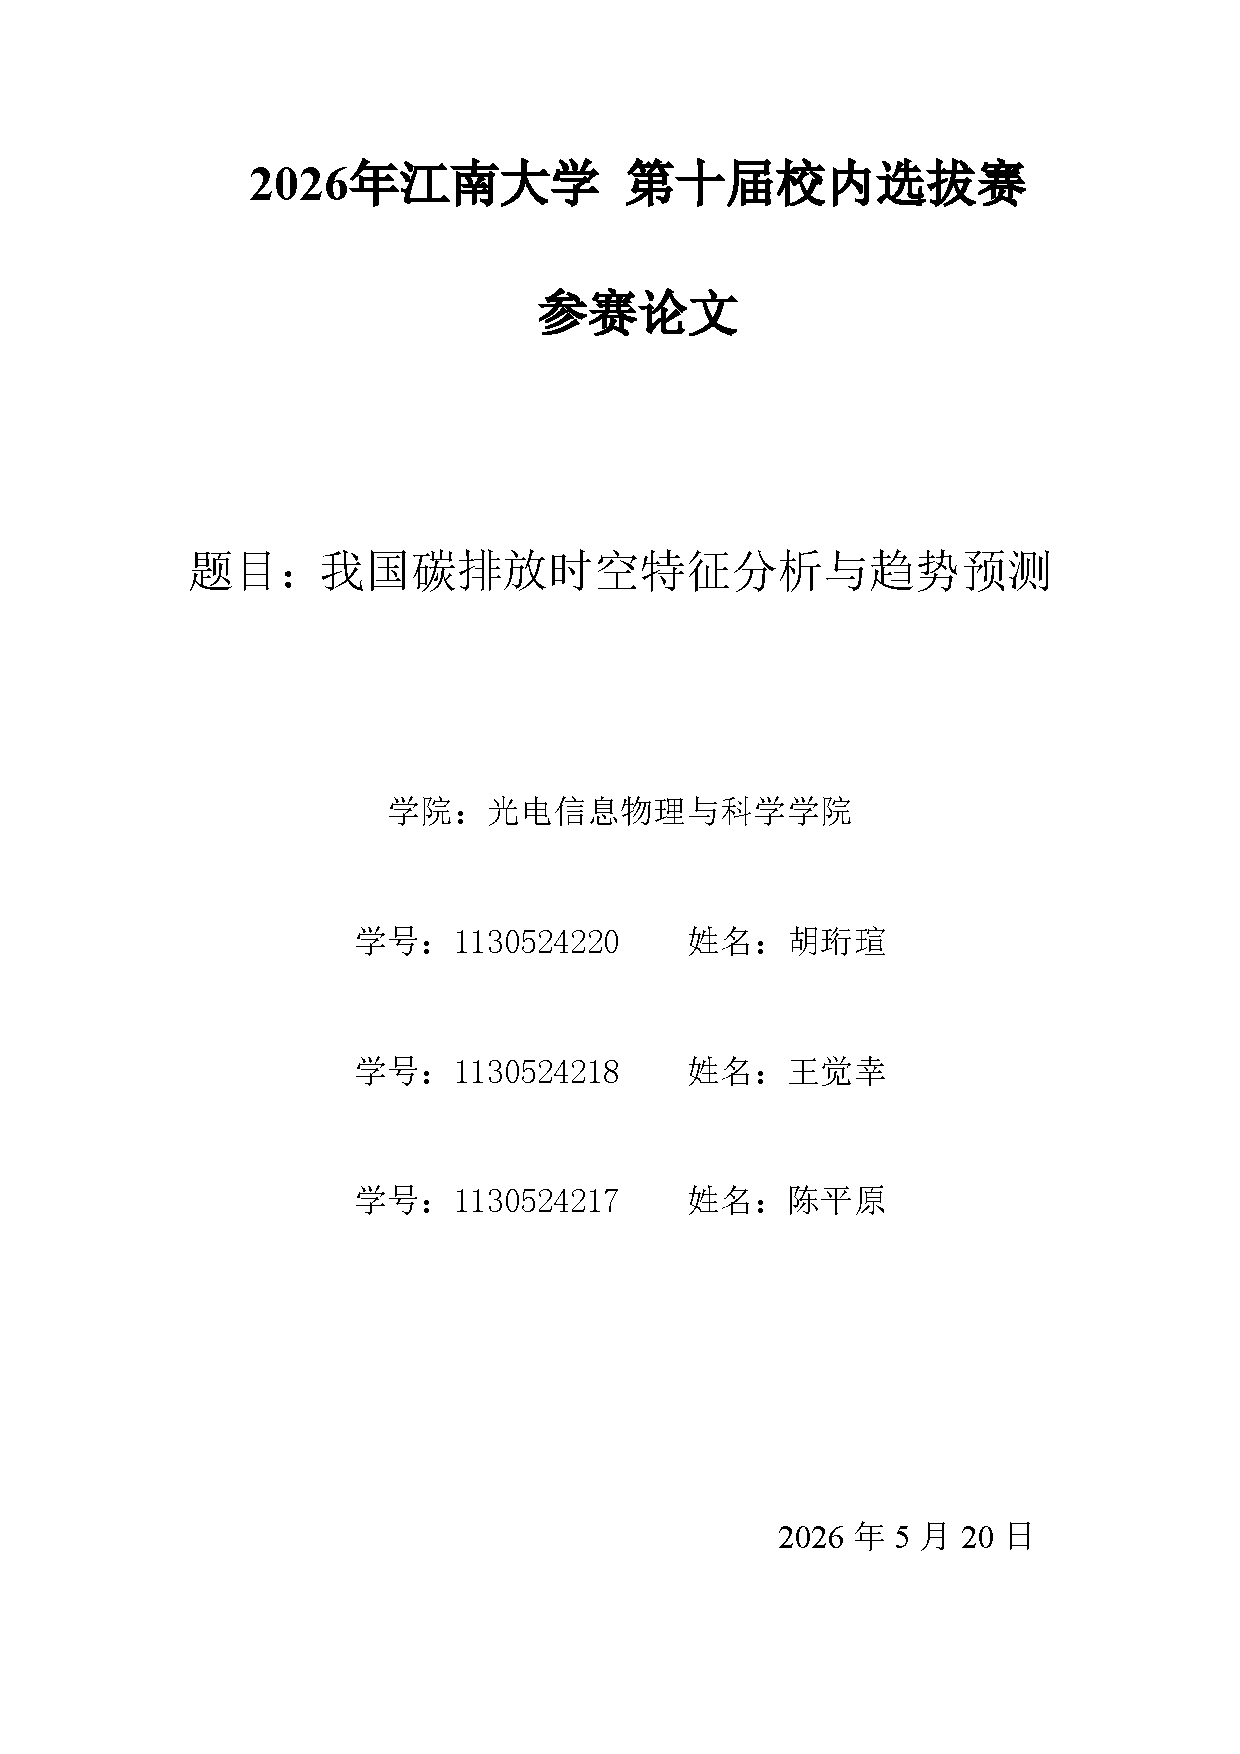
\includepdf[pages=1,pagecommand={\thispagestyle{empty}}]{assets/第一页封面.pdf}

\clearpage
\setcounter{page}{1}

\begin{center}
{\heiti\zihao{3} 我国碳排放时空特征分析与趋势预测}
\end{center}

\begin{center}
{\heiti\zihao{4} 摘要}
\end{center}

碳达峰、碳中和是我国推进高质量发展和生态文明建设的重要战略目标，也与能源供应、产业升级和居民低碳生活密切相关。不同地区资源禀赋、产业基础和发展阶段差异明显，导致省际碳排放水平和减排压力并不均衡。研究我国碳排放时空特征、影响因素和未来趋势，有助于为区域差异化减排和“双碳”政策实施提供量化依据。

{\heiti 对于问题一}，首先基于2022年30省碳排放清单，选取CO$_2$总量、人均CO$_2$、碳排放强度、煤炭相关排放占比等指标进行统计分析，并结合省级空间分布结果识别高排放集聚区域。其次，设各省低碳综合评价得分为决策变量$S_i$，建立{\heiti 熵权 TOPSIS}综合评价模型；进一步构造{\heiti K-means 聚类}模型，对省份进行分类分级。模型采用Python实现并求解。结果表明，我国省际碳排放呈现“北方资源能源高排放带、东部沿海制造业高排放带、中西南相对低排放区”的格局；山东、内蒙古、河北、江苏、山西、广东、河南、辽宁是排放总量最高的省份。资源依赖高排放型省份主要包括河北、山西、内蒙古、宁夏、新疆，应重点控煤和推动资源型产业转型；北京、上海属于经济发达效率型，可承担技术示范和绿色金融引领功能。

{\heiti 对于问题二}，首先围绕能源消费结构、产业结构、人均GDP、城镇化率和人口规模等因素分析碳排放驱动机制。其次，设碳排放总量$C_i$为因变量，人口规模$P_i$、人均GDP$A_i$、煤炭相关排放占比$Coal_i$、第二产业占比$IS_i$、城镇化率$U_i$为解释变量，建立{\heiti STIRPAT 模型}，并采用{\heiti OLS}估计、{\heiti VIF}检验和{\heiti 岭回归}稳健性检验。结果表明，当前省际碳排放差异最主要由人口规模和煤炭依赖共同驱动，其中煤炭相关排放占比是最关键、最稳定的结构性因素；人均GDP、第二产业占比和城镇化率的影响更多通过能源结构和产业结构间接体现。因此，单纯压缩经济活动并非合理路径，降低煤炭占比、推进重点行业节能降碳、提升经济产出效率才是控制排放的核心方向。

{\heiti 对于问题三}，首先以2024年全国实际排放量11901.44 Mt为基准，分析2026--2045年全国碳排放趋势。其次，将问题二得到的{\heiti STIRPAT 模型}系数转化为年度递推模型，设置基准、低碳、强化低碳三种{\heiti 情景预测}方案，并以人口增长率、人均GDP增长率、煤炭占比变化、第二产业占比变化和城镇化率变化作为情景参数。模型采用Python递推求解并进行灵敏度分析。结果表明，若维持基准转型速度，全国可能在2032年左右达峰，峰值约12435 Mt，达峰偏晚且峰值较高；低碳情景可将达峰时间提前到2026年左右，2045年排放降至8903 Mt；强化低碳情景下降幅最大，2045年排放约7114 Mt，较峰值下降40.2\%。因此，实现更早达峰和更大减排潜力的关键在于加快煤炭替代、优化产业结构并提高单位GDP产出效率。

{\heiti 对于问题四}，在前三问结果基础上，本文从区域分类、关键驱动因素和情景预测结论出发提出差异化减排方案。结果表明，资源依赖高排放型省份应以控煤、煤电改造和新能源基地建设为重点；工业制造高排放型省份应优先推进钢铁、建材、电力、石化等行业节能降碳；中等转型压力型省份应严控高耗能产业转移；北京、上海等效率型地区应发挥绿色金融、碳交易和技术示范作用。总体看，降低煤炭占比和提高产业效率是兼顾达峰时间与减排潜力的核心政策抓手。

\vfill

\noindent{\heiti 关键词：熵权 TOPSIS；K-means 聚类；STIRPAT 模型；情景预测}

\clearpage


\section*{一、问题重述}

\subsection*{1.1 问题背景}

全球气候变暖已成为人类社会面临的共同挑战，极端天气、能源安全和产业转型压力不断加大，控制温室气体排放已成为各国经济社会发展的重要议题。我国提出碳达峰、碳中和目标，要求在保障经济增长和居民生活质量的同时，持续推进能源结构调整、产业低碳升级和绿色生活方式转变。由于我国不同省份在资源禀赋、人口规模、产业结构、能源结构和经济发展水平方面差异明显，碳排放总量、排放效率和减排压力也表现出显著的空间不均衡性。因此，准确刻画省际碳排放分布特征，识别排放增长的关键驱动因素，并预测未来碳排放变化趋势，对于制定差异化、可考核、可持续的区域减排政策具有重要现实意义。

\begin{figure}[H]
  \centering
  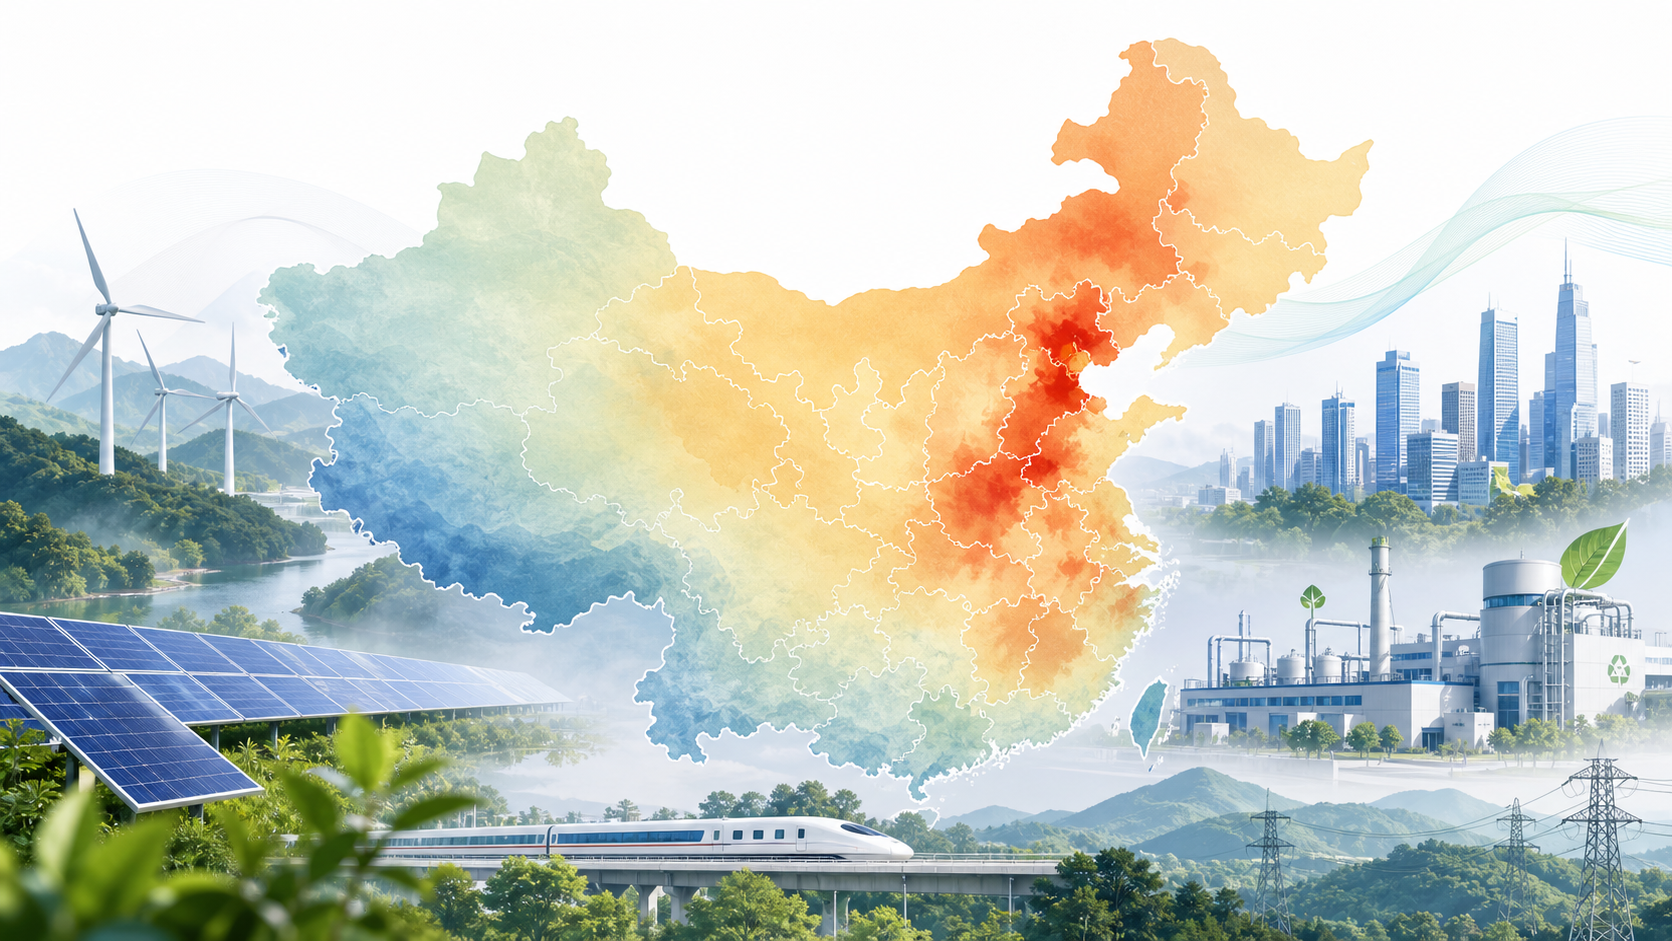
\includegraphics[width=0.82\textwidth]{assets/fig0_background_carbon.png}
  \caption{碳排放空间差异与绿色转型背景示意图}
\end{figure}

\subsection*{1.2 问题提出}

为了服务我国区域差异化减排和碳达峰路径研判，现需结合题目附件和相关统计资料建立数学模型，重点分析以下问题：

\begin{itemize}
  \item {\heiti 问题一：}选取碳排放总量、人均碳排放、碳排放强度等核心指标，分析30个省份碳排放的空间分布特征和差异显著性，并在此基础上建立省份分类分级模型。
  \item {\heiti 问题二：}从能源消费结构、产业结构、人均GDP、城镇化率、人口规模等因素中识别影响碳排放的核心驱动因素，构建定量模型并完成参数估计、显著性检验和模型优化。
  \item {\heiti 问题三：}基于前述驱动因素模型，设置基准、低碳、强化低碳三种发展情景，预测2026--2045年全国碳排放总量与碳排放强度变化趋势，判断碳达峰时间节点、峰值水平和减排潜力。
  \item {\heiti 问题四：}综合省份分类结果、驱动因素识别结果和情景预测结论，提出具有区域针对性和可操作性的减排政策建议。
\end{itemize}

\section*{二、问题分析}

\subsection*{2.1 问题一的分析}

问题一需要回答两个递进层面。首先，要判断各省碳排放是否存在明显的空间分布特征和差异显著性，这不仅要比较排放总量，还要结合地理位置观察高排放区域是否呈现集聚现象。其次，要在差异分析基础上对省份进行分类分级，使结果能够服务于后续政策建议。若只比较CO$_2$总量，容易把人口规模大、经济总量大的省份简单判定为高排放压力省份，而忽视其单位人口排放、单位经济产出排放和能源结构差异。因此，问题一需要同时兼顾排放规模、排放效率、能源依赖和经济发展基础。

为此，本文选取CO$_2$总量、人均CO$_2$、碳排放强度、煤炭相关排放占比、第二产业占比、人均GDP和城镇化率作为核心指标。先通过省级空间热力图直观呈现排放的地理集聚格局，再用变异系数、基尼系数和泰尔指数刻画省际差异显著性；随后构建熵权TOPSIS模型，利用客观权重得到各省低碳发展综合得分；最后采用K-means聚类对省份进行分类，使“空间分布--差异测度--综合评价--分类分级”形成完整分析链条。

\subsection*{2.2 问题二的分析}

问题二的核心是从多个候选因素中识别碳排放的主要驱动因素，并建立能够解释省际排放差异的定量模型。碳排放通常受到人口规模、经济活动水平、产业结构、能源消费结构和城镇化进程共同影响，这些因素之间并非相互独立。例如，人口规模扩大会推高能源需求，人均GDP提高会改变消费和生产活动强度，第二产业占比较高通常意味着更强的能源消耗，煤炭占比较高则会直接提高单位能源消费对应的碳排放。因此，模型不仅要估计各因素的方向和强弱，还要检验变量间相关性对结论稳定性的影响。

为此，本文采用STIRPAT模型作为问题二的基本框架，将碳排放总量对人口、人均GDP、煤炭相关排放占比、第二产业占比和城镇化率的弹性关系转化为对数线性回归模型。模型参数采用OLS估计，并通过回归系数、标准误、t统计量和$p$值判断变量影响方向及显著性；同时引入VIF检验多重共线性，避免解释变量高度相关造成误判。考虑到省级横截面样本量有限，进一步采用岭回归和留一交叉验证作为稳健性检验，从而判断驱动因素识别结论是否可靠。

\subsection*{2.3 问题三的分析}

问题三要求在未来较长时期内预测全国碳排放总量和碳排放强度，并进一步判断碳达峰时间、峰值水平和减排潜力。该问题不同于前两问的横截面分析，它需要把驱动因素的影响关系转化为年度变化路径。由于全国年度样本较短，若直接建立复杂多变量时间序列模型，容易出现参数不稳定和外推误差较大的问题。同时，未来人口、经济增长、能源结构和产业结构本身具有不确定性，单一路径预测难以反映不同政策强度下的排放差异。

为此，本文以2024年全国实际排放量作为预测基准，将问题二得到的STIRPAT弹性系数转化为年度相对变化递推模型，使人口增长率、人均GDP增长率、煤炭占比变化率、第二产业占比变化率和城镇化率变化率共同决定下一期排放水平。在情景设置上，分别构建基准、低碳和强化低碳三种发展路径，以体现不同能源替代速度和产业转型强度。最后根据各情景预测序列识别峰值年份和峰值排放量，并计算2045年相对峰值的减排比例；同时进行单因素和组合扰动灵敏度分析，检验关键参数变化对预测结论的影响。

\subsection*{2.4 问题四的分析}

问题四要求在前三问定量分析基础上提出政策建议，因此它不是简单的文字总结，而是需要把空间差异、分类分级、驱动因素和未来情景预测连接起来。不同类型省份的排放压力来源并不相同：资源依赖型地区主要受煤炭消费和能源结构制约，工业制造型地区更多受高耗能行业和产业结构影响，经济发达效率型地区则具备技术、资金和治理优势。若采用统一政策口径，容易造成高排放省份减排压力不足或低排放省份承担过高转型成本。

为此，本文将问题一得到的省份类型作为政策分区依据，将问题二识别出的煤炭相关排放占比、人口规模等关键驱动因素作为政策抓手，并结合问题三中三种情景下的达峰时间和减排潜力判断政策强度。政策建议按照“资源依赖高排放型、工业制造高排放型、中等转型压力型、经济发达效率型”分别提出，重点围绕控煤降碳、重点行业节能改造、防止高耗能产业转移、绿色金融和碳市场机制展开，从而形成具有区域针对性和可操作性的减排路径。

\section*{三、模型假设}

1. 附件中碳排放数据真实可靠，各省统计口径在同一年份内具有可比性。

2. 2022年省级横截面数据能够代表当前我国省际碳排放差异和主要结构特征。

3. 人口规模、经济发展水平、能源结构、产业结构和城镇化率是影响碳排放的重要因素，且可通过STIRPAT模型进行定量刻画。

4. 全国中长期碳排放趋势主要由人口、人均经济水平、煤炭占比、产业结构和城镇化率共同决定。

5. 情景预测中，各驱动变量变化率在2026--2045年间平滑变化，不考虑突发重大外部冲击。

6. 附件1中2025年全国碳排放数据截至2025年9月30日，不能直接作为完整年度数据与2019--2024年比较，预测基准采用2024年全国排放量。

\section*{四、符号说明}

\begin{table}[H]
\centering
\caption{主要符号说明}
\begin{tabularx}{0.92\textwidth}{cXc}
\toprule
符号 & 说明 & 单位 \\
\midrule
$C_i$ & 第$i$个省份碳排放总量 & Mt \\
$P_i$ & 第$i$个省份人口规模 & 万人 \\
$GDP_i$ & 第$i$个省份地区生产总值 & 亿元 \\
$PC_i$ & 第$i$个省份人均碳排放 & 吨/人 \\
$CI_i$ & 第$i$个省份碳排放强度 & 吨/万元GDP \\
$Coal_i$ & 第$i$个省份煤炭相关排放占比 & \% \\
$IS_i$ & 第$i$个省份第二产业占比 & \% \\
$A_i$ & 第$i$个省份人均GDP & 万元/人 \\
$U_i$ & 第$i$个省份城镇化率 & \% \\
$z_{ij}$ & 第$i$个省份第$j$个指标标准化值 & -- \\
$w_j$ & 第$j$个评价指标权重 & -- \\
$S_i$ & 第$i$个省份TOPSIS综合贴近度 & -- \\
$G$ & 基尼系数 & -- \\
$T$ & 泰尔指数 & -- \\
$CV$ & 变异系数 & -- \\
$g_P$ & 人口增长率 & \% \\
$g_A$ & 人均GDP增长率 & \% \\
$\Delta Coal$ & 煤炭相关排放占比变化量 & 百分点 \\
$\Delta IS$ & 第二产业占比变化量 & 百分点 \\
$\Delta U$ & 城镇化率变化量 & 百分点 \\
\bottomrule
\end{tabularx}
\end{table}

\section*{六、问题一的模型建立与求解}

\subsection*{6.1 指标选取与基础变量构造}

问题一要求同时回答“空间差异是否显著”和“省份应如何分类分级”。为避免只用排放总量造成片面判断，本文从排放规模、人口压力、经济效率、能源结构、产业结构和发展水平六个方面构建指标体系。具体变量包括碳排放总量（$C_i$）、人口规模（$P_i$）、地区生产总值（$GDP_i$）、人均碳排放（$PC_i$）、碳排放强度（$CI_i$）、煤炭相关排放占比（$Coal_i$）、第二产业占比（$IS_i$）、人均GDP（$A_i$）和城镇化率（$U_i$）。其中，$C_i$反映排放规模，$PC_i$反映居民平均排放压力，$CI_i$反映单位经济产出的排放效率，$Coal_i$和$IS_i$分别反映能源结构与产业结构，$A_i$和$U_i$反映发展水平和治理基础。

在原始变量基础上，首先构造人均碳排放、碳排放强度和人均GDP三个派生指标：
\[
\left\{
\begin{aligned}
PC_i&=\frac{C_i}{P_i},\\
CI_i&=\frac{C_i}{GDP_i},\\
A_i&=\frac{GDP_i}{P_i}.
\end{aligned}
\right.
\]
第一式表示第$i$省的居民平均排放水平；第二式表示单位GDP对应的碳排放量，数值越低说明经济产出效率越高；第三式表示第$i$省的经济发展水平。这样处理后，可以将人口规模和经济规模差异从总量指标中分离出来，使省际比较更公平。

\subsection*{6.2 空间差异测度模型}

为判断省际碳排放差异是否显著，本文对核心指标$x_i$分别计算变异系数、基尼系数和泰尔指数。变异系数用于衡量相对离散程度，基尼系数用于衡量省际分布不均衡程度，泰尔指数可进一步刻画差异强度。设$x_i$表示第$i$省某一碳排放指标，$\mu_x$和$\sigma_x$分别为该指标的均值和标准差，则变异系数为
\[
CV=\frac{\sigma_x}{\mu_x}.
\]
当$CV$较大时，说明各省之间相对差异明显。

将$x_i$按从小到大排序后，基尼系数定义为
\[
G=\frac{2\sum_{i=1}^{n}ix_i}{n\sum_{i=1}^{n}x_i}-\frac{n+1}{n}.
\]
该式通过排序后各省指标值的累积分布刻画不均衡程度，$G$越大，说明指标越集中于少数省份。

泰尔指数定义为
\[
T=\frac{1}{n}\sum_{i=1}^{n}\frac{x_i}{\bar{x}}\ln\left(\frac{x_i}{\bar{x}}\right).
\]
其中，$\bar{x}$为指标均值。当某些省份指标值显著高于均值时，泰尔指数会增大，因此可作为差异显著性的补充度量。

\subsection*{6.3 熵权TOPSIS综合评价模型}

空间差异指标只能说明“差异有多大”，不能直接判断各省低碳发展水平的综合优劣。因此，本文进一步构建熵权TOPSIS模型[1]。设第$i$省第$j$个指标的原始值为$x_{ij}$，评价指标集合为
\[
X_i=(C_i,PC_i,CI_i,Coal_i,IS_i,A_i,U_i).
\]
其中，$C_i$、$PC_i$、$CI_i$、$Coal_i$和$IS_i$越小越有利于低碳发展，作为负向指标；$A_i$和$U_i$体现经济基础和城市治理能力，作为正向指标。

首先对指标进行无量纲化处理。正向指标和负向指标分别采用如下标准化公式：
\[
z_{ij}=
\begin{cases}
\dfrac{x_{ij}-\min_i x_{ij}}{\max_i x_{ij}-\min_i x_{ij}}, & \text{正向指标},\\[8pt]
\dfrac{\max_i x_{ij}-x_{ij}}{\max_i x_{ij}-\min_i x_{ij}}, & \text{负向指标}.
\end{cases}
\]
该式把不同量纲的指标统一映射到$[0,1]$区间，并保证数值越大代表低碳表现越好。

然后计算熵权。令$p_{ij}=z_{ij}/\sum_{i=1}^{n}z_{ij}$，则第$j$个指标的熵值和权重分别为
\[
e_j=-\frac{1}{\ln n}\sum_{i=1}^{n}p_{ij}\ln p_{ij},\qquad
w_j=\frac{1-e_j}{\sum_{j=1}^{m}(1-e_j)}.
\]
熵值$e_j$越小，说明该指标在省际之间差异越明显、提供的信息量越大，因此对应权重$w_j$越高。

最后计算各省到理想解和负理想解的距离。设$z_j^+=\max_i z_{ij}$为理想解，$z_j^-=\min_i z_{ij}$为负理想解，则
\[
D_i^+=\sqrt{\sum_{j=1}^{m}w_j(z_{ij}-z_j^+)^2},\qquad
D_i^-=\sqrt{\sum_{j=1}^{m}w_j(z_{ij}-z_j^-)^2}.
\]
据此得到TOPSIS贴近度
\[
S_i=\frac{D_i^-}{D_i^++D_i^-}.
\]
$S_i$越接近1，表示第$i$省越接近低碳理想状态；$S_i$越接近0，说明其排放压力或结构压力越大。

\subsection*{6.4 K-means分类模型}

在得到综合评价结果后，还需要将省份划分为若干具有政策含义的类型。本文采用K-means聚类算法[2]，仍以$X_i=(C_i,PC_i,CI_i,Coal_i,IS_i,A_i,U_i)$作为聚类变量。该变量组同时覆盖排放规模、排放效率、能源结构、产业结构和发展基础，能够反映不同省份减排压力来源的差异。

设$G_k$为第$k$类省份集合，$\mu_k$为第$k$类中心，聚类目标为最小化类内平方误差和：
\[
J=\sum_{k=1}^{K}\sum_{i\in G_k}\|X_i-\mu_k\|^2.
\]
当$J$越小时，同一类型内部省份越相似。为辅助判断聚类数$K$，本文计算轮廓系数
\[
s(i)=\frac{b(i)-a(i)}{\max\{a(i),b(i)\}}.
\]
其中，$a(i)$为省份$i$与同类省份的平均距离，$b(i)$为省份$i$与最近其他类省份的平均距离。$s(i)$越接近1，说明该省份分类越合理。

\subsection*{6.5 求解结果与分析}

基于2022年30省数据，首先计算空间差异指标，结果如表\ref{tab:spatial}所示。

\begin{table}[H]
\centering
\caption{省际碳排放空间差异指标}
\label{tab:spatial}
\small
\begin{tabular}{lrrrrrr}
\toprule
指标 & 均值 & 变异系数 & 基尼系数 & 泰尔指数 & 最小值 & 最大值 \\
\midrule
CO$_2$总量/Mt & 380.2822 & 0.6458 & 0.3549 & 0.2041 & 44.6919 & 920.9053 \\
人均CO$_2$/吨每人 & 9.8017 & 0.7957 & 0.3513 & 0.2312 & 3.2763 & 36.6002 \\
碳排放强度/吨每万元GDP & 1.3011 & 0.7958 & 0.3883 & 0.2555 & 0.1720 & 4.8805 \\
煤炭相关排放占比 & 0.7113 & 0.2510 & 0.1263 & 0.0447 & 0.0212 & 0.9399 \\
\bottomrule
\end{tabular}
\end{table}

结合图\ref{fig:map}可以看出，2022年我国30省碳排放呈现明显地理集聚特征。高排放区域集中在华北--环渤海及内蒙古能源基地一带，东部沿海制造业省份也形成高排放带，中西部和西南多数省份排放总量相对较低。因此，省际碳排放空间格局可概括为“北方资源能源高排放带、东部沿海制造业高排放带、中西南相对低排放区、局部资源型高值点”。

\begin{figure}[H]
\centering
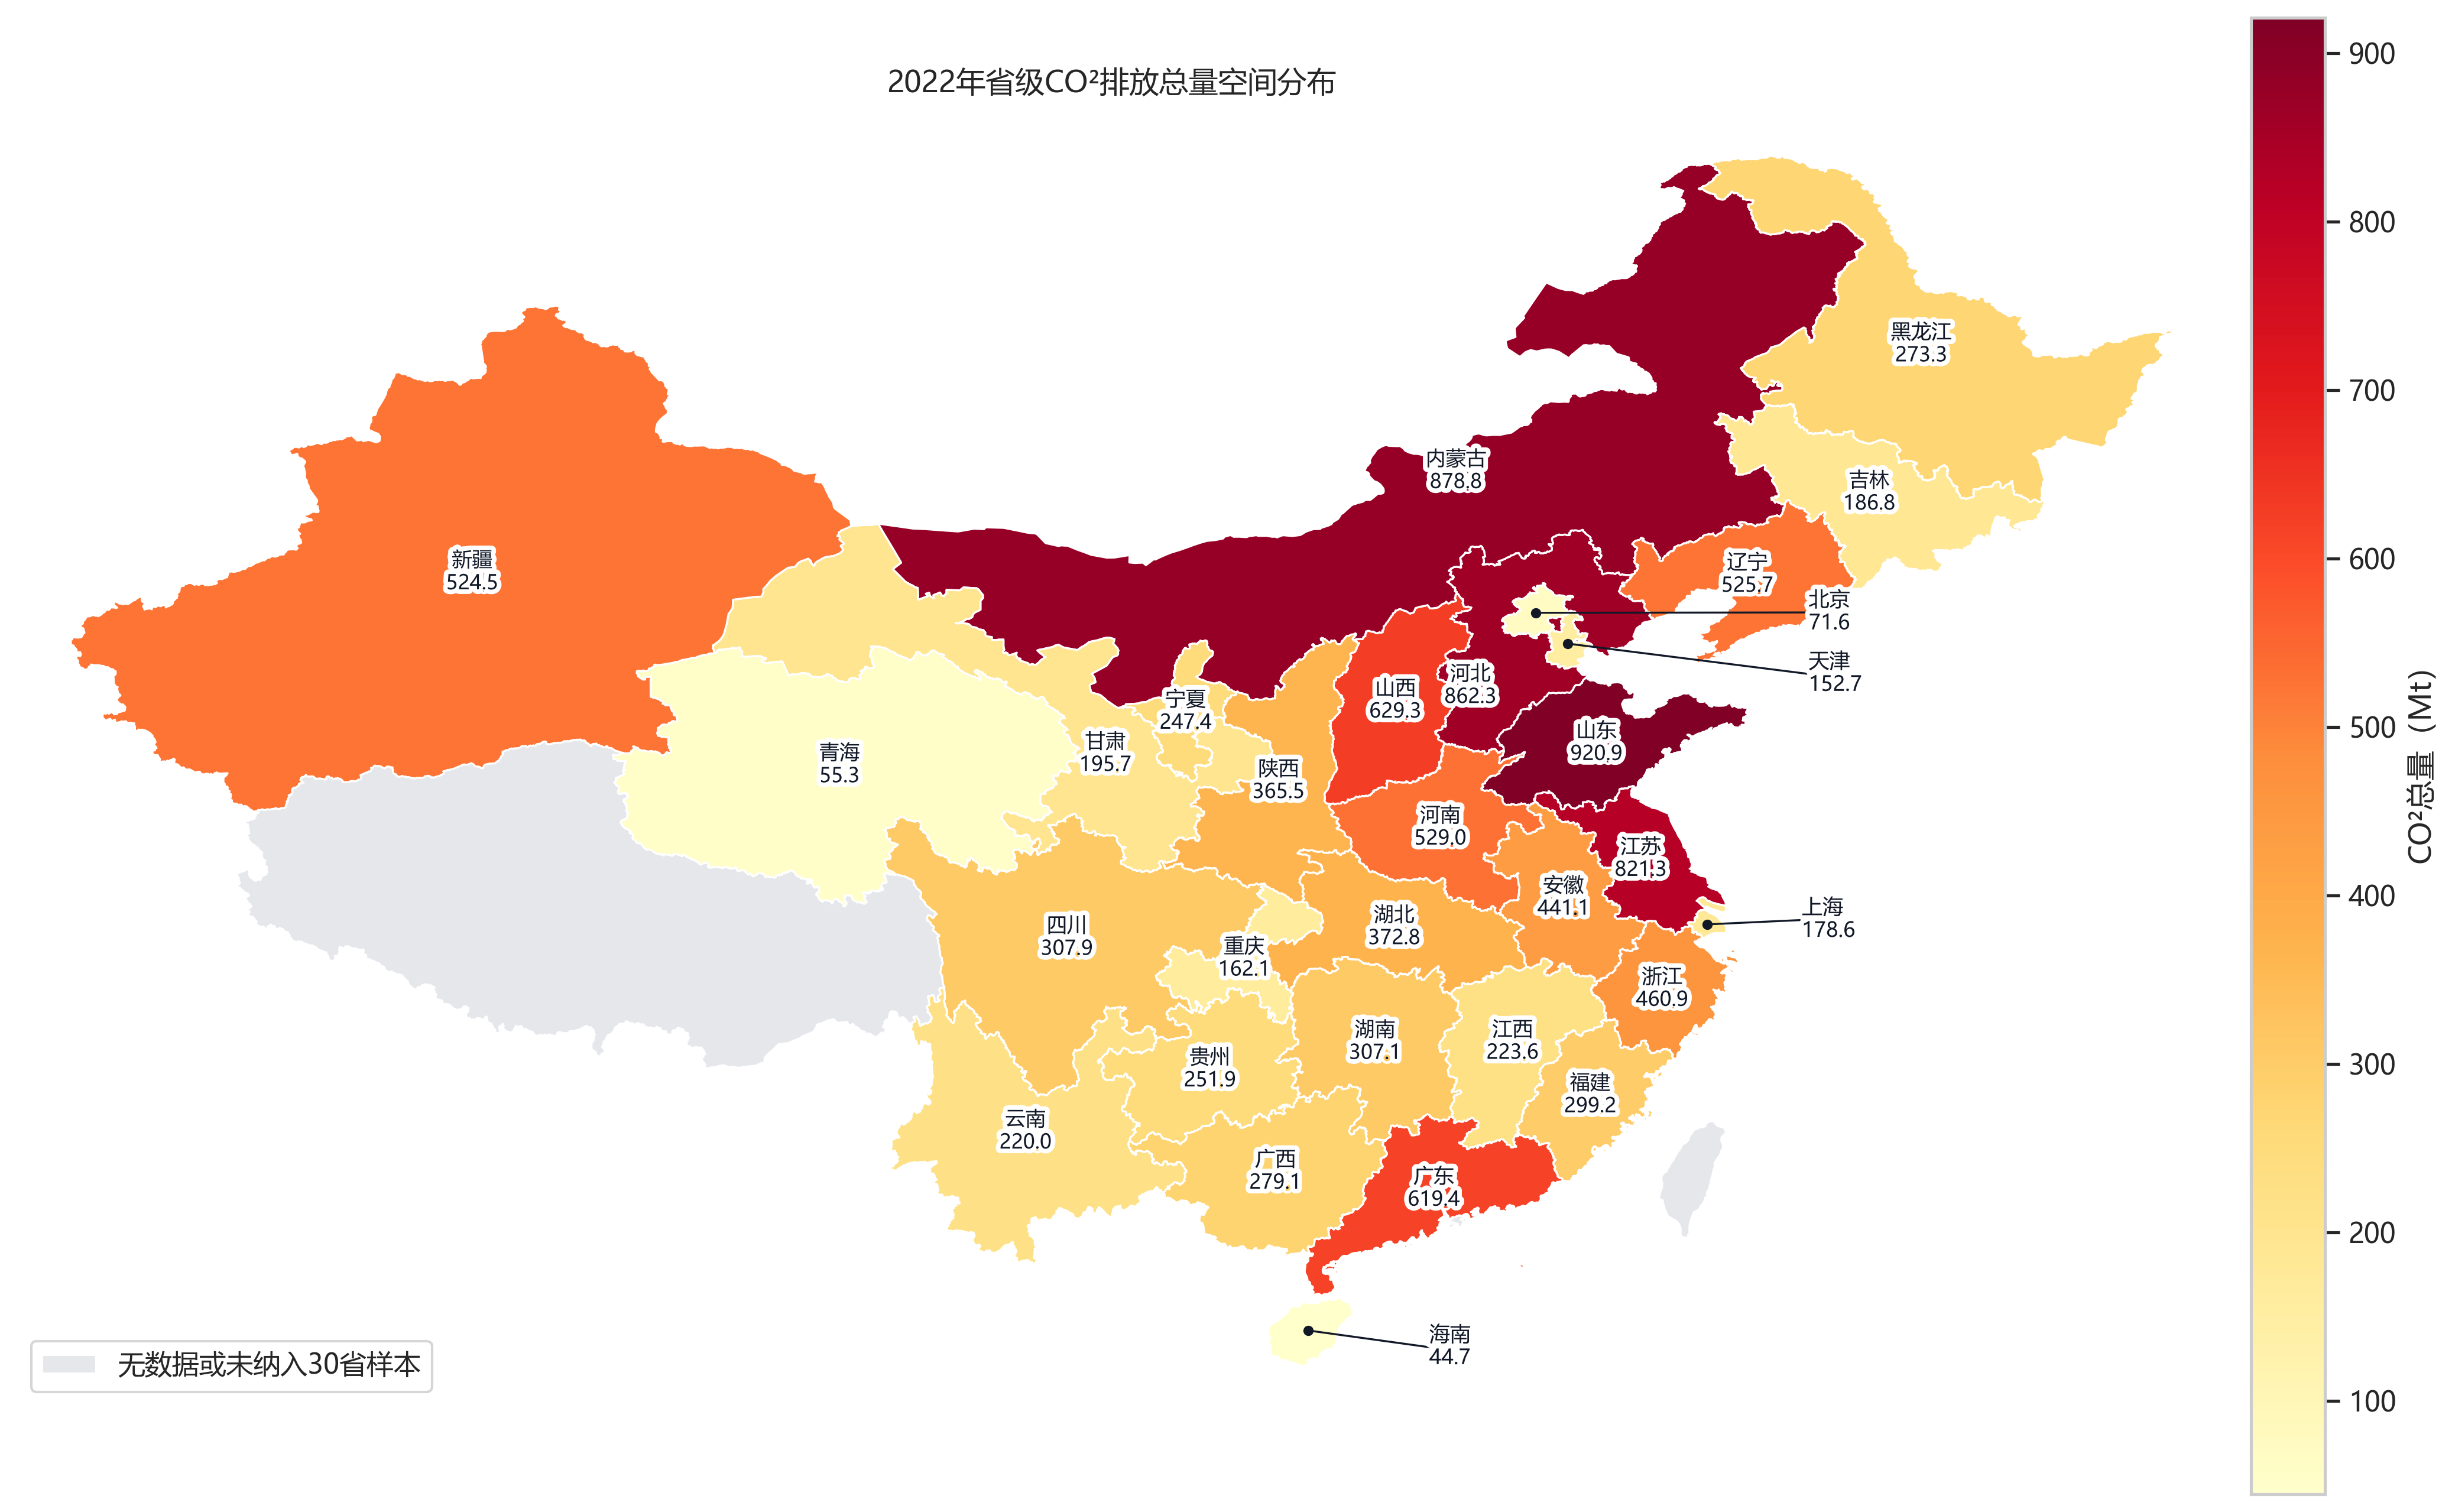
\includegraphics[width=0.94\textwidth]{assets/fig1_map.png}
\caption{2022年省级CO$_2$排放总量空间分布热力图}
\label{fig:map}
\end{figure}

差异显著性方面，2022年30省CO$_2$总量均值为380.2822 Mt，但最大值山东为920.9053 Mt，最小值海南为44.6919 Mt，二者相差约20.61倍；排放总量前8位省份合计占30省总排放的50.72\%，说明排放明显集中在少数重点省份。碳排放强度基尼系数为0.3883，高于总量基尼系数，说明省际排放效率差异更突出。

熵权TOPSIS评价结果显示，指标权重前三位为人均GDP、煤炭相关排放占比和城镇化率，权重分别为0.2728、0.2215和0.1717。TOPSIS得分排名靠前的省份为北京、上海、天津、海南、浙江、福建、重庆、广东；排名靠后的省份为山西、内蒙古、新疆、河北、宁夏、河南、山东、甘肃。聚类模型中K=3时轮廓系数最高，但K=4能够更清晰地区分资源依赖、工业制造、中等转型和经济发达效率型省份，政策解释性更强。因此本文采用K=4作为最终分类，结果如表\ref{tab:cluster}所示。

\begin{table}[H]
\centering
\caption{K-means聚类分类结果}
\label{tab:cluster}
\begin{tabularx}{\textwidth}{p{3.2cm}p{7.1cm}X}
\toprule
类型 & 省份 & 结果分析 \\
\midrule
资源依赖高排放型 & 河北、山西、内蒙古、宁夏、新疆 & 煤炭占比和排放强度高，减排重点是控煤和资源型产业转型 \\
工业制造高排放型 & 天津、辽宁、江苏、浙江、福建、山东、湖北、广东、重庆、陕西 & 排放总量较高，减排重点是重点行业节能改造 \\
中等转型压力型 & 吉林、黑龙江、安徽、江西、河南、湖南、广西、海南、四川、贵州、云南、甘肃、青海 & 总量和强度居中，需防止高耗能产业转移 \\
经济发达效率型 & 北京、上海 & 排放强度低，适合发挥技术、金融和治理优势 \\
\bottomrule
\end{tabularx}
\end{table}

\section*{七、问题二的模型建立与求解}

\subsection*{7.1 驱动因素选择}

问题二要求识别影响碳排放的核心驱动因素，并建立可检验的定量模型。结合STIRPAT理论和省级数据可得性，本文以碳排放总量（$C_i$）为被解释变量，选取人口规模（$P_i$）、人均GDP（$A_i$）、煤炭相关排放占比（$Coal_i$）、第二产业占比（$IS_i$）和城镇化率（$U_i$）作为解释变量。人口规模（$P_i$）代表社会经济活动总量，人均GDP（$A_i$）代表富裕程度和消费生产强度，煤炭相关排放占比（$Coal_i$）代表能源结构，第二产业占比（$IS_i$）代表产业结构，城镇化率（$U_i$）代表发展阶段和城市能源需求。

\subsection*{7.2 STIRPAT模型构建}

STIRPAT模型由IPAT恒等式扩展而来[3]，本文将其写为
\[
I=aP^bA^cT^d e.
\]
式中，$I$表示环境影响，本文对应碳排放总量；$P$表示人口规模；$A$表示富裕程度；$T$表示技术和结构因素；$a$为常数项，$b,c,d$为弹性系数，$e$为随机扰动项。由于能源结构、产业结构和城镇化率难以合并为单一技术变量，本文将$T$拆分为$Coal_i$、$IS_i$和$U_i$三个可观测变量。

对模型两边取对数，并结合省级横截面数据，得到本文的扩展STIRPAT模型：
\[
\ln C_i=\alpha+\beta_1\ln P_i+\beta_2\ln A_i+\beta_3Coal_i+\beta_4IS_i+\beta_5U_i+\varepsilon_i.
\]
其中，$\beta_1$表示人口规模对碳排放的弹性，$\beta_2$表示人均GDP对碳排放的弹性；$\beta_3$、$\beta_4$和$\beta_5$分别表示煤炭占比、第二产业占比和城镇化率变化对碳排放对数值的边际影响。若某一系数为正，说明该因素增加会推动碳排放上升；若为负，则说明该因素具有抑制排放的作用。

\subsection*{7.3 参数估计与模型检验}

令$y_i=\ln C_i$，$\hat{y}_i$为模型拟合值，OLS估计通过最小化残差平方和得到参数：
\[
\hat{\boldsymbol\beta}_{OLS}=\arg\min_{\boldsymbol\beta}\sum_{i=1}^{n}(y_i-\hat{y}_i)^2.
\]
该方法使预测值与真实值之间的总体误差最小，用于获得STIRPAT主模型参数。

考虑到解释变量之间可能存在相关性，本文进一步计算方差膨胀因子：
\[
VIF_j=\frac{1}{1-R_j^2}.
\]
其中，$R_j^2$为第$j$个解释变量对其余解释变量回归得到的决定系数。$VIF_j$越大，说明该变量与其他解释变量相关性越强，多重共线性风险越高。

为检验模型稳健性，本文采用岭回归作为补充。岭回归目标函数为
\[
\hat{\boldsymbol\beta}_{ridge}
=\arg\min_{\boldsymbol\beta}\left\{\sum_{i=1}^{n}(y_i-\hat{y}_i)^2+\lambda\sum_{j=1}^{p}\beta_j^2\right\}.
\]
其中，$\lambda$为惩罚系数。该式在残差平方和基础上加入系数平方惩罚，可以降低多重共线性和小样本波动对参数估计的影响。

\subsection*{7.4 求解结果与分析}

估计结果见表\ref{tab:ols}。模型$R^2$为0.8762，调整$R^2$为0.8504，RMSE\_log为0.2672，F检验$p$值为$3.919\times10^{-10}$，说明模型对省际碳排放差异具有较强解释力。

\begin{table}[H]
\centering
\caption{STIRPAT模型OLS估计结果}
\label{tab:ols}
\begin{tabular}{lrrrr}
\toprule
变量 & 系数 & 标准误 & t值 & p值 \\
\midrule
$\ln P$ & 0.6447 & 0.0807 & 7.9856 & 0.0000 \\
$\ln A$ & 0.4502 & 0.3860 & 1.1663 & 0.2549 \\
煤炭相关排放占比 & 2.8275 & 0.5798 & 4.8770 & 0.0001 \\
第二产业占比 & 0.5080 & 1.1516 & 0.4412 & 0.6630 \\
城镇化率 & 0.8029 & 1.3461 & 0.5965 & 0.5565 \\
\bottomrule
\end{tabular}
\end{table}

从参数估计结果看，人口规模和煤炭相关排放占比对碳排放具有显著正向影响。其中，$\ln P$系数为0.6447，煤炭相关排放占比系数为2.8275，且二者$p$值较小，是当前样本中最稳定的排放驱动因素。VIF检验显示所有解释变量VIF均小于10，不存在严重多重共线性。岭回归留一交叉验证得到LOOCV\_$R^2$为0.7851，说明模型具有一定预测稳健性。

\begin{figure}[H]
\centering
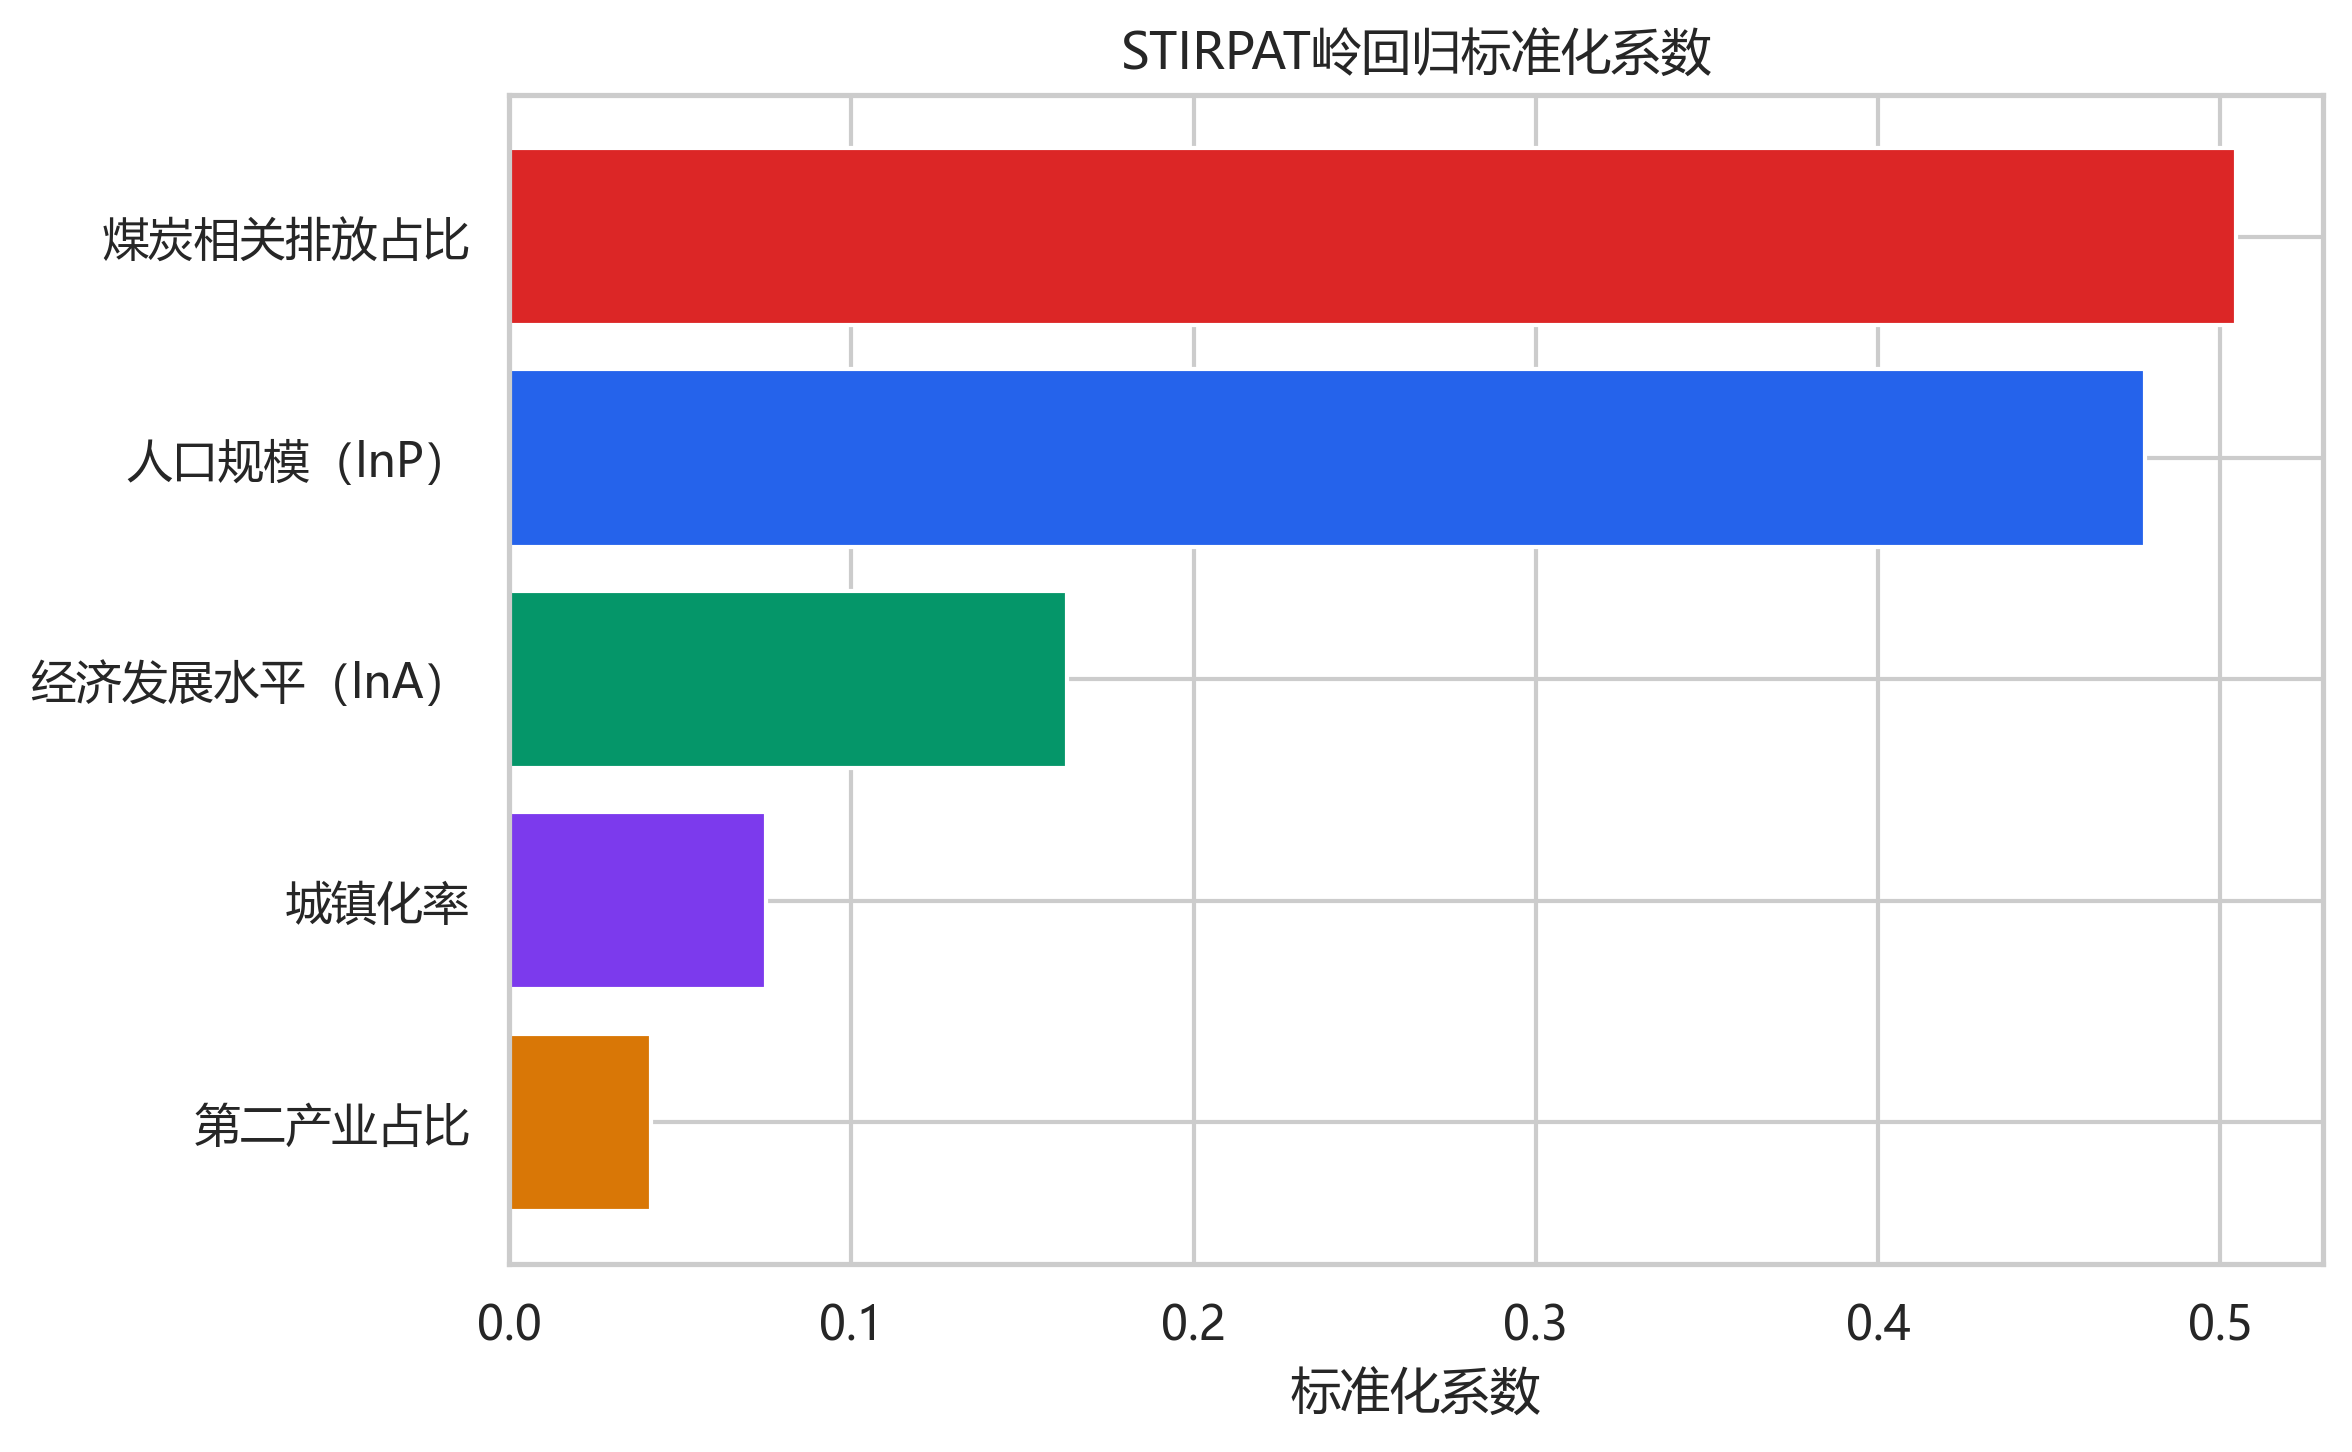
\includegraphics[width=0.82\textwidth]{assets/fig4_stirpat_coef.png}
\caption{STIRPAT岭回归标准化系数}
\label{fig:coef}
\end{figure}

\begin{figure}[H]
\centering
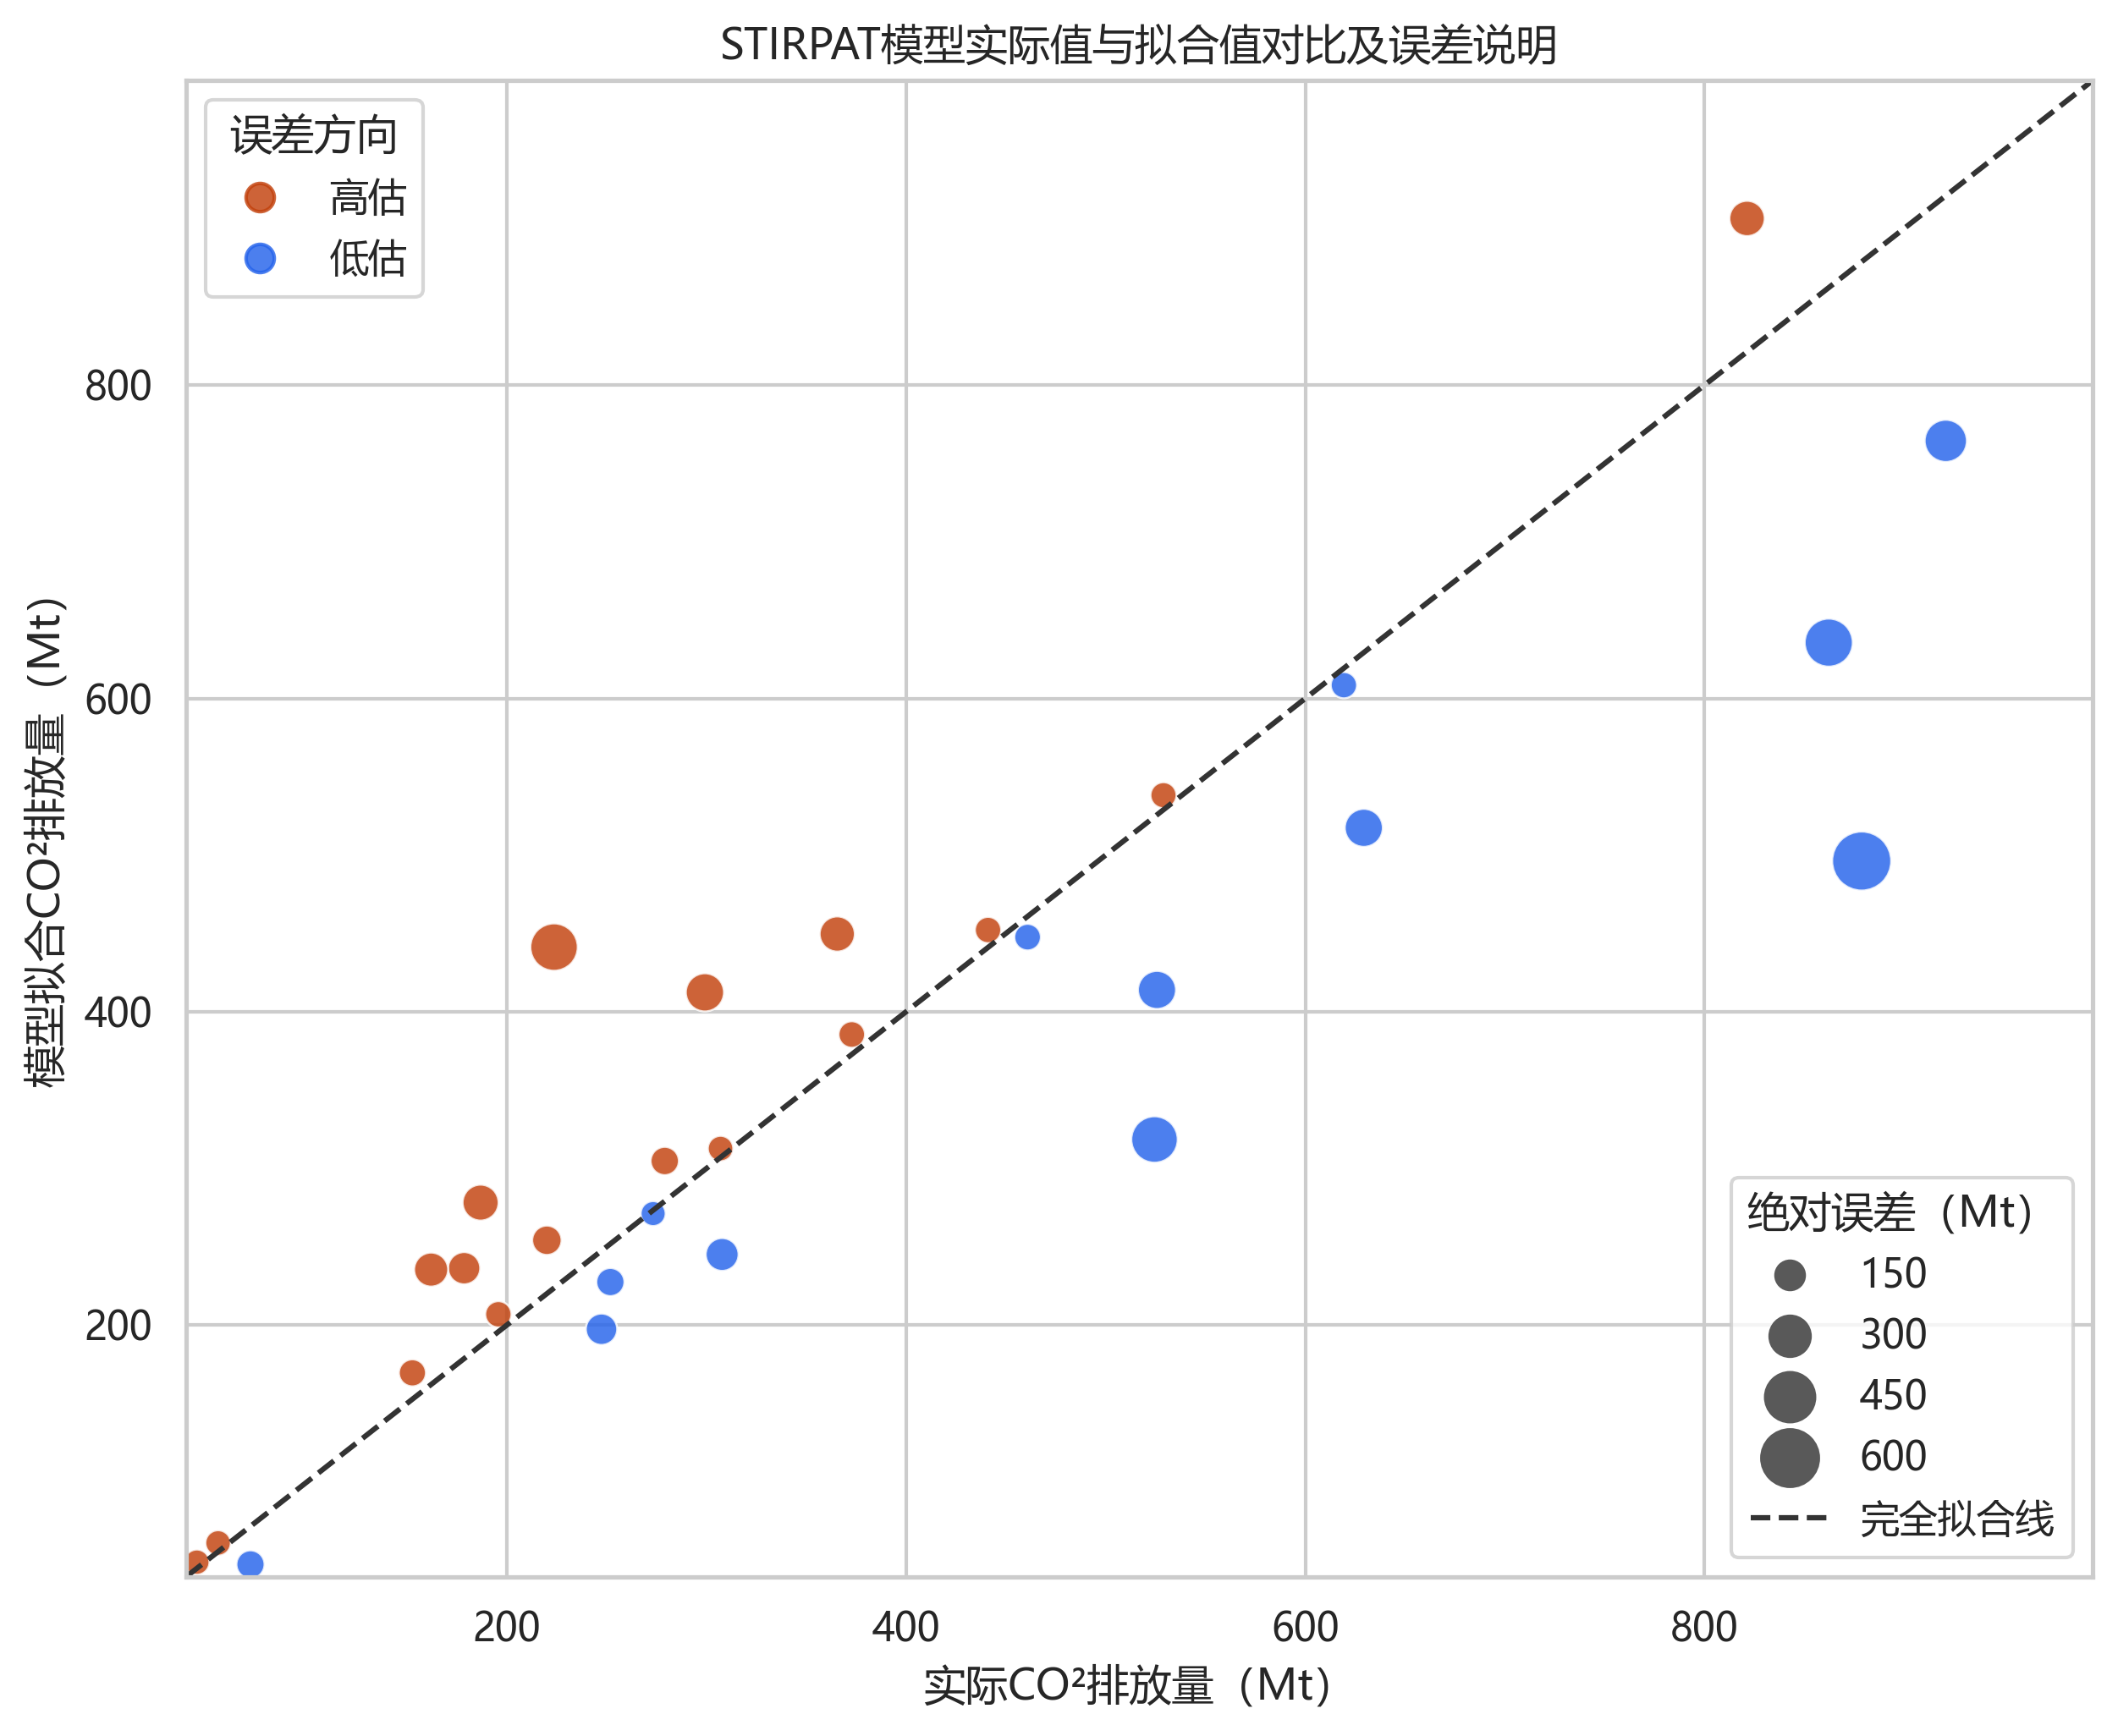
\includegraphics[width=0.82\textwidth]{assets/fig5_ols_fit.png}
\caption{OLS拟合值与真实值对比}
\label{fig:olsfit}
\end{figure}

\section*{八、问题三的模型建立与求解}

\subsection*{8.1 预测变量与建模思路}

问题三要求预测2026--2045年全国碳排放总量与强度，并判断达峰时间、峰值水平和减排潜力。与问题二的省级横截面模型不同，问题三需要把驱动因素关系转化为年度递推过程。本文使用全国碳排放总量（$C_t$）、人口规模（$P_t$）、人均GDP（$A_t$）、煤炭相关排放占比（$Coal_t$）、第二产业占比（$IS_t$）和城镇化率（$U_t$）作为预测变量。其中，$P_t$和$A_t$反映人口与经济增长，通常会推高排放；$Coal_t$和$IS_t$反映能源结构和产业结构，是低碳转型的主要调节变量；$U_t$反映城镇化发展阶段。

由于全国年度样本较短，直接建立多变量时间序列回归会使参数不稳定。因此，本文沿用问题二得到的STIRPAT系数，将其转化为相对变化递推模型。该做法的含义是：未来某一年排放变化不是单独由时间趋势决定，而是由人口、经济、能源结构、产业结构和城镇化率的年度变化共同决定。

\subsection*{8.2 STIRPAT递推预测模型}

设$\Delta\ln C_t=\ln C_t-\ln C_{t-1}$，$\Delta Coal_t=Coal_t-Coal_{t-1}$，其余变量类似，则年度排放变化由下式给出：
\[
\Delta\ln C_t=\beta_1\Delta\ln P_t+\beta_2\Delta\ln A_t+\beta_3\Delta Coal_t+\beta_4\Delta IS_t+\beta_5\Delta U_t.
\]
该式把问题二估计得到的驱动因素系数用于年度变化分析：人口和人均GDP采用对数变化率，煤炭占比、第二产业占比和城镇化率采用比例变化量。

由$\Delta\ln C_t$可以递推出下一年排放总量：
\[
\left\{
\begin{aligned}
C_t&=C_{t-1}\exp(\Delta\ln C_t),\\
GDP_t&=P_tA_t,\\
CI_t&=\frac{C_t}{GDP_t}.
\end{aligned}
\right.
\]
第一式表示以$t-1$年排放总量为基础，根据驱动因素变化得到$t$年排放；第二式表示全国GDP由人口和人均GDP相乘得到；第三式表示碳排放强度，即单位GDP对应的碳排放量。

达峰年份和减排潜力定义为
\[
Y_{peak}=\arg\max_t C_t,\qquad
R_{2045}=1-\frac{C_{2045}}{\max_t C_t}.
\]
其中，$Y_{peak}$表示预测期内排放总量达到最大值的年份；$R_{2045}$表示2045年相对峰值排放的下降比例，数值越大说明减排潜力越充分。

\subsection*{8.3 情景参数设置}

全国年度碳排放总量仅使用附件1中$Sector=Total$统计。2019--2024年全国碳排放整体处于高位波动状态，2024年为11901.44 Mt。2025年只有273天记录，不能作为完整年度值进行同比比较。因此，本文以2024年全国排放量11901.44 Mt作为情景预测基准。三种情景参数设置见表\ref{tab:scenario_params}。

基准情景假设现有转型速度延续，经济保持中速增长，煤炭占比和第二产业占比逐步下降；低碳情景假设能源替代和产业优化速度进一步提高；强化低碳情景假设政策约束、技术进步和非化石能源替代力度显著增强。三种情景均保持人口增长率逐步下降的趋势，以反映我国人口变化现实。

\begin{table}[H]
\centering
\caption{三情景参数设置}
\label{tab:scenario_params}
\scriptsize
\begin{tabularx}{\textwidth}{lXXXXX}
\toprule
情景 & 人口增长率 & 人均GDP增长率 & 煤炭占比年变化 & 第二产业占比年变化 & 城镇化率年变化 \\
\midrule
基准情景 & -0.10\%$\rightarrow$-0.20\% & 4.50\%$\rightarrow$2.60\% & -0.40$\rightarrow$-1.00百分点 & -0.05$\rightarrow$-0.20百分点 & 0.35$\rightarrow$0.15百分点 \\
低碳情景 & -0.10\%$\rightarrow$-0.20\% & 4.30\%$\rightarrow$2.40\% & -0.60$\rightarrow$-1.40百分点 & -0.10$\rightarrow$-0.30百分点 & 0.30$\rightarrow$0.10百分点 \\
强化低碳情景 & -0.10\%$\rightarrow$-0.25\% & 4.10\%$\rightarrow$2.20\% & -0.80$\rightarrow$-1.80百分点 & -0.20$\rightarrow$-0.50百分点 & 0.25$\rightarrow$0.05百分点 \\
\bottomrule
\end{tabularx}
\end{table}

\subsection*{8.4 预测结果与检验}

预测结果见表\ref{tab:peak}和图\ref{fig:scenario}。基准情景下，碳排放在2032年达到约12435 Mt峰值，随后缓慢下降，2045年较峰值下降11.4\%。低碳情景下，排放约在2026年达到峰值11959 Mt，2045年较峰值下降25.6\%。强化低碳情景下降幅最大，2045年降至7114 Mt，较峰值下降40.2\%。

\begin{table}[H]
\centering
\caption{三情景达峰与减排潜力}
\label{tab:peak}
\scriptsize
\begin{tabular}{lrrrrrr}
\toprule
情景 & 达峰年份 & 峰值/Mt & 2030年/Mt & 2035年/Mt & 2045年/Mt & 2045较峰值下降 \\
\midrule
低碳情景 & 2026 & 11959 & 11829 & 11229 & 8903 & 25.6\% \\
基准情景 & 2032 & 12435 & 12404 & 12351 & 11014 & 11.4\% \\
强化低碳情景 & 2024 & 11901 & 11258 & 10165 & 7114 & 40.2\% \\
\bottomrule
\end{tabular}
\end{table}

\begin{figure}[H]
\centering
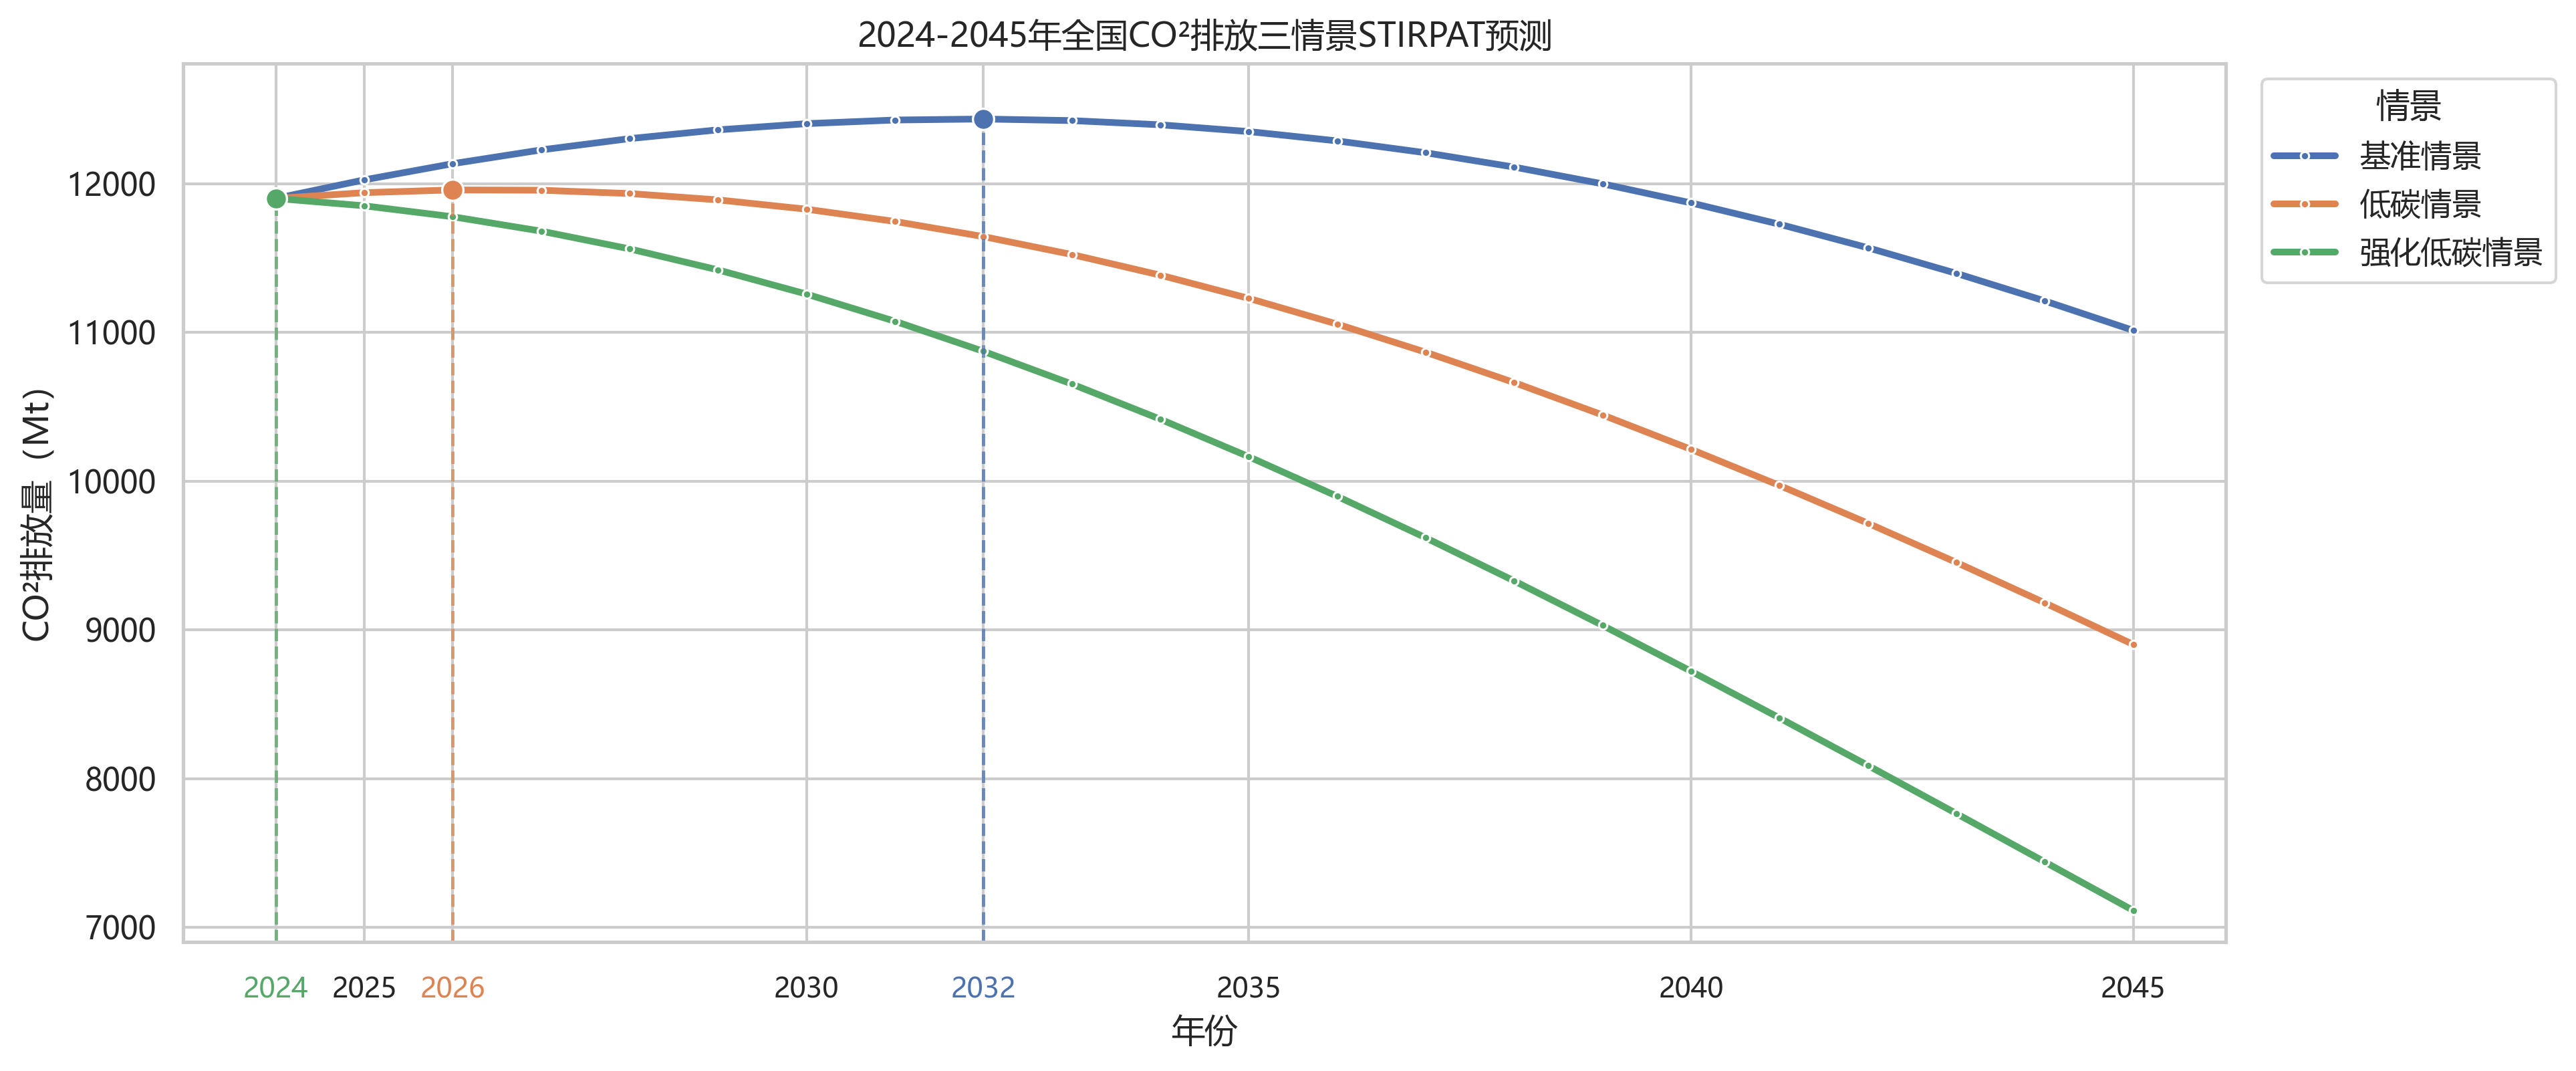
\includegraphics[width=0.88\textwidth]{assets/fig6_scenario.png}
\caption{2024--2045年三情景碳排放趋势}
\label{fig:scenario}
\end{figure}

灵敏度分析表明，2045年排放量对煤炭占比下降速度和人均GDP增长率最敏感。当煤炭占比下降速度减弱20\%时，2045年排放量增加约954.7 Mt，达峰年份推迟至2035年；当煤炭占比下降速度增强20\%时，2045年排放量减少约878.6 Mt，达峰年份提前至2030年。主要结论在合理扰动范围内未发生根本改变，说明模型具有一定稳健性。

\begin{figure}[H]
\centering
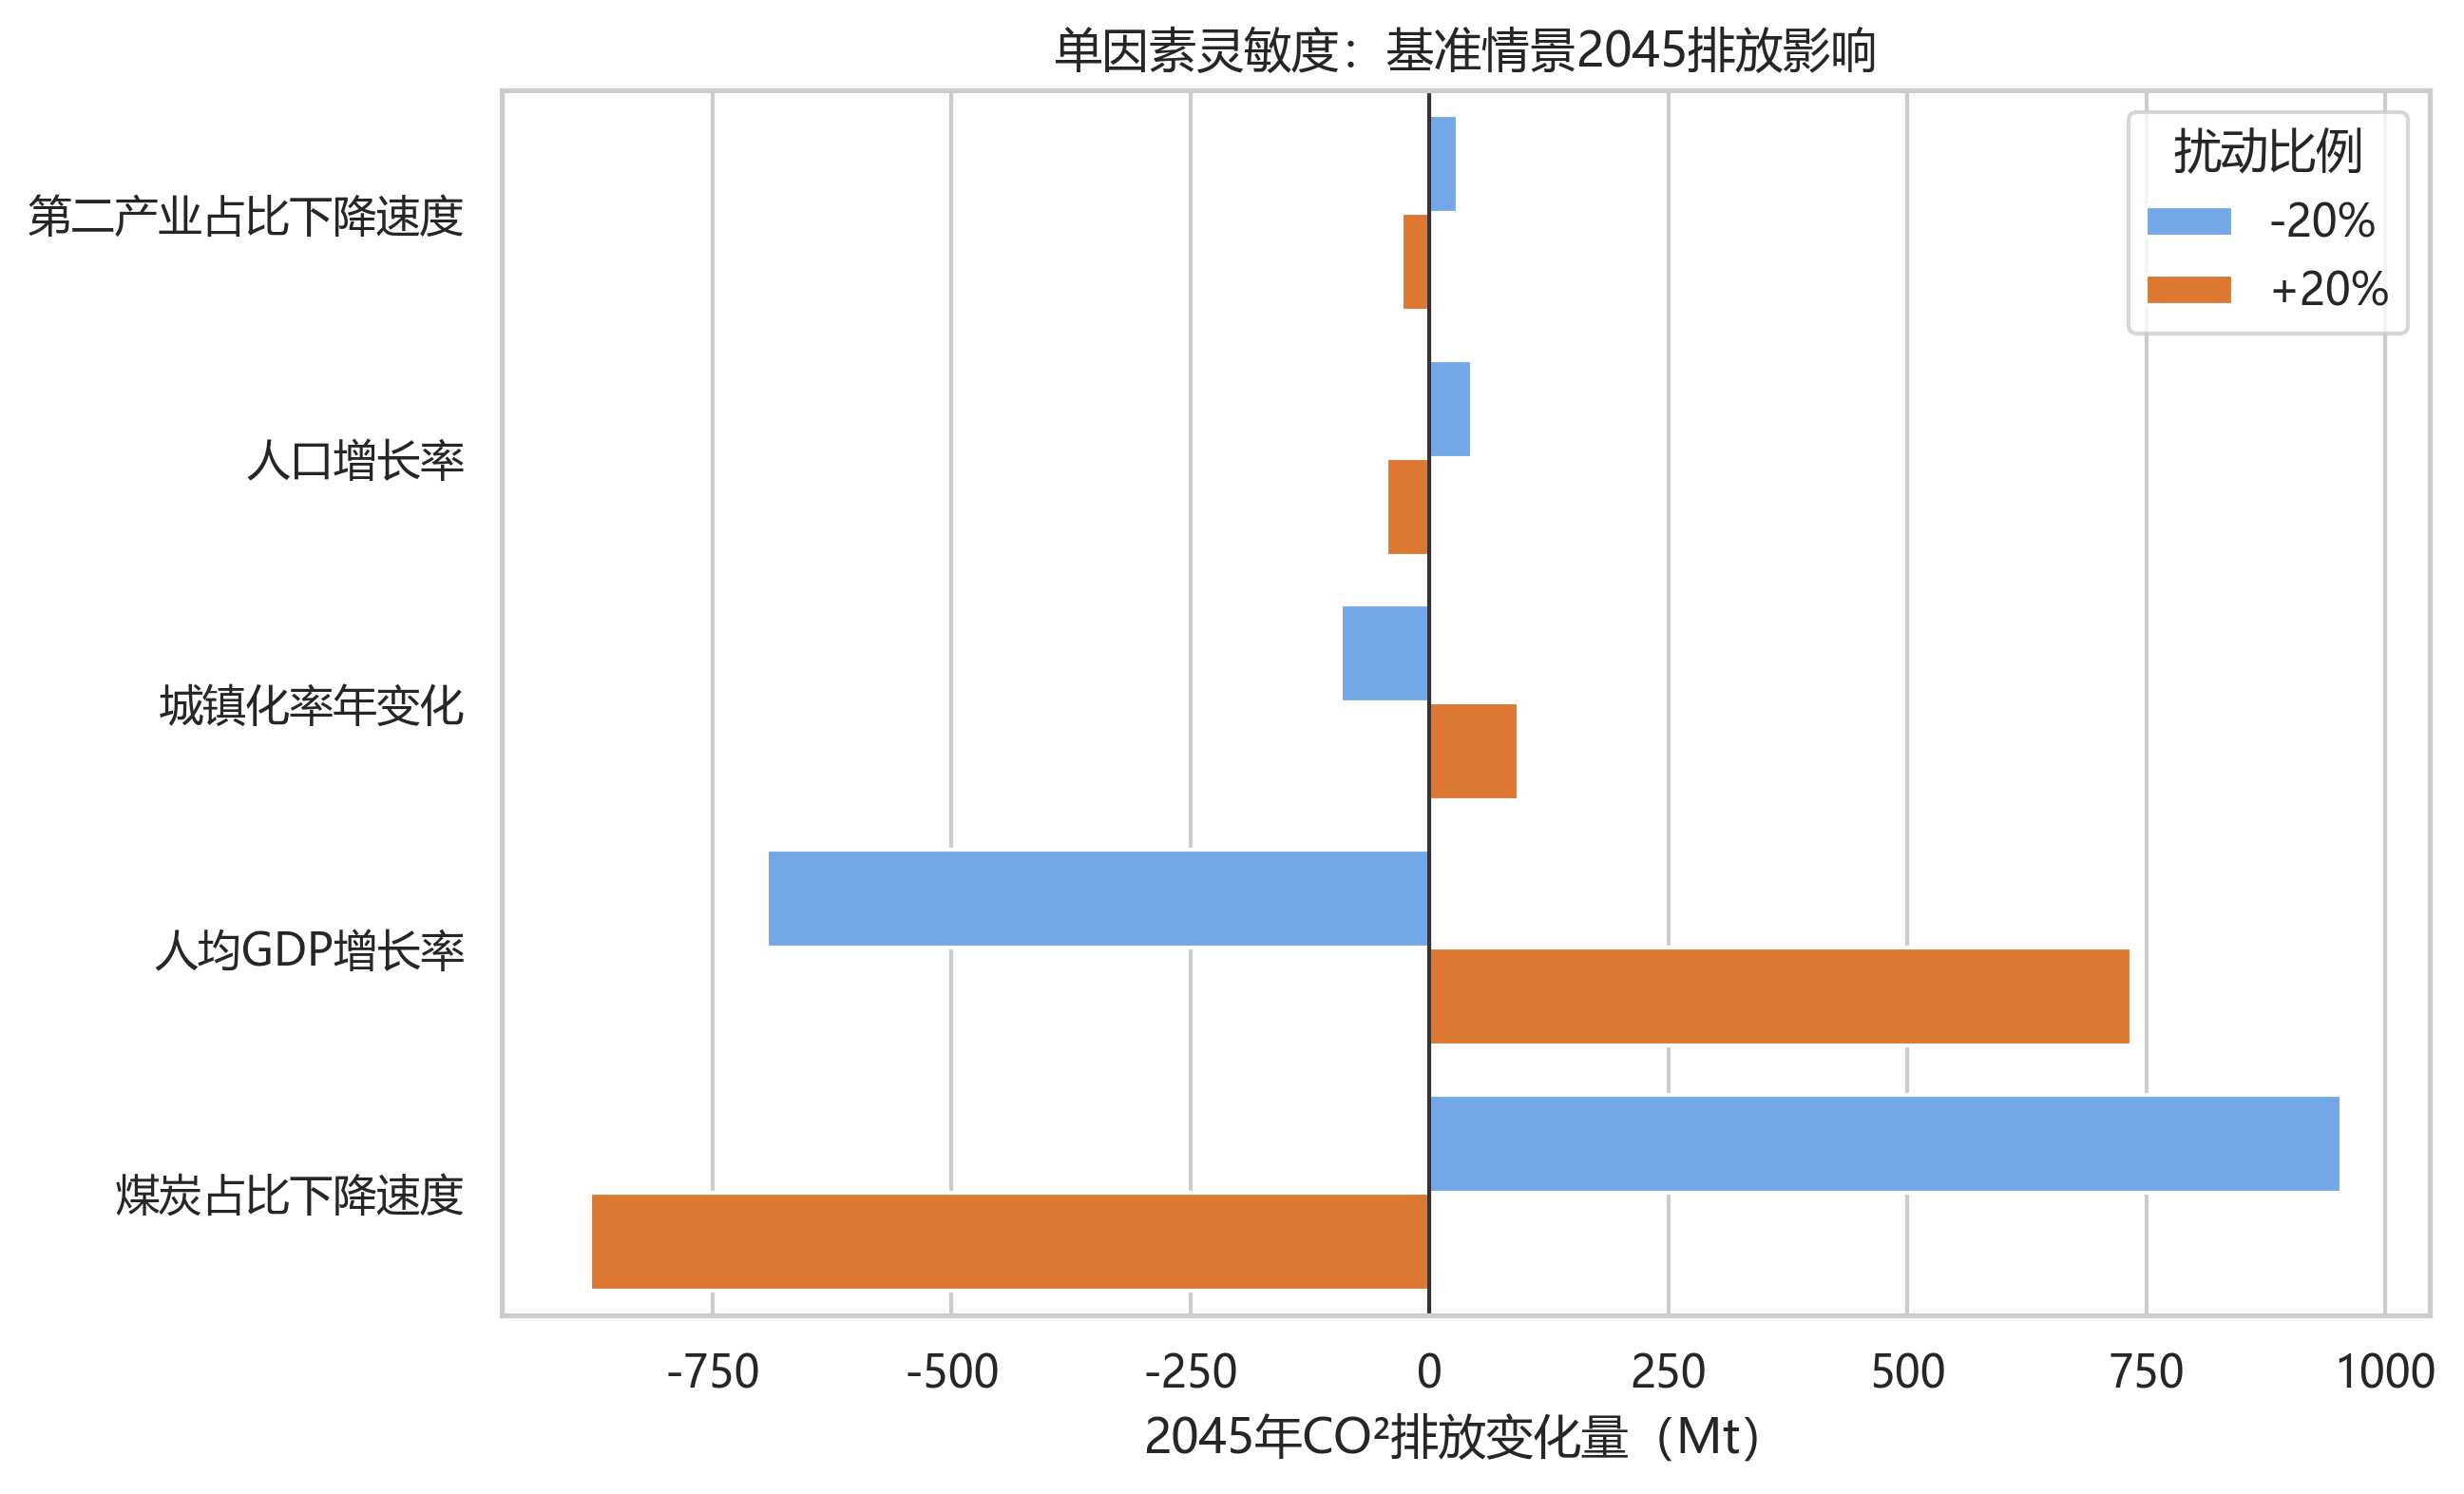
\includegraphics[width=0.84\textwidth]{assets/fig8_sensitivity.png}
\caption{单因素灵敏度对2045年排放的影响}
\label{fig:sensitivity}
\end{figure}

\subsection*{8.5 政策建议归纳}

基于前三问结果，建议资源依赖高排放型省份重点控制煤炭消费总量并推进资源型产业转型；工业制造高排放型省份聚焦钢铁、建材、电力、石化和交通等重点行业节能改造；中等转型压力型省份防止高耗能产业简单转移；经济发达效率型地区发挥绿色金融、碳交易和技术创新优势。全国层面应持续降低煤炭占比，扩大非化石能源供给，强化技术创新和碳市场机制。

\section*{九、模型的评价与改进}

\subsection*{9.1 模型的优点}

1. 模型体系完整。本文从空间差异、综合评价、分类分级、驱动因素识别、趋势预测和政策建议六个层面展开，能够完整回应题目要求。

2. 解释性较强。熵权TOPSIS、K-means聚类和STIRPAT模型均具有较清晰的经济含义，便于解释不同省份的低碳发展水平和排放驱动机制。

3. 结果展示直观。空间差异指标、TOPSIS排名、聚类类型、回归系数和情景预测结果都通过表格和图形呈现，便于比较和分析。

4. 情景预测逻辑稳定。STIRPAT递推模型将问题二估计得到的驱动因素系数直接用于问题三预测，使驱动因素识别与中长期趋势研判形成衔接。

\subsection*{9.2 模型的缺点}

1. 省级建模主要基于2022年横截面数据，尚不能充分刻画各省碳排放随时间变化的动态机制。若能补充多年省级面板数据，可进一步建立双向固定效应STIRPAT模型。

2. STIRPAT模型采用线性对数形式，难以反映复杂非线性关系和变量之间的交互效应。后续可尝试空间计量模型或非线性机器学习模型进行补充检验。

3. 情景预测依赖参数设定，不同参数组合会影响达峰年份和减排潜力判断。本文已通过灵敏度分析检验主要结论稳健性，但未来仍可进一步扩大参数组合范围。

4. 当前模型主要分析省际差异，没有进一步考虑相邻地区之间的空间溢出效应。后续可引入空间自相关检验和空间杜宾模型，对区域联动减排进行深入研究。

\section*{参考文献}

[1] Deng H，Yeh C H，Willis R J，Inter-company comparison using modified TOPSIS with objective weights，Computers \& Operations Research，27(10)：963-973，2000。

[2] MacQueen J，Some methods for classification and analysis of multivariate observations，Proceedings of the Fifth Berkeley Symposium on Mathematical Statistics and Probability，1：281-297，1967。

[3] York R，Rosa E A，Dietz T，STIRPAT, IPAT and ImPACT: analytic tools for unpacking the driving forces of environmental impacts，Ecological Economics，46(3)：351-365，2003。

\clearpage
\section*{附录}

本文计算结果由Python程序统一生成。附录列出核心程序，包括总入口脚本、公共函数和问题一至问题四的求解脚本。

\subsection*{附录A 总入口脚本 run\_all.py}
\VerbatimInput[fontsize=\tiny,breaklines=true,breakanywhere=true,numbers=left,frame=single]{assets/code/run_all.py}

\subsection*{附录B 公共函数 common.py}
\VerbatimInput[fontsize=\tiny,breaklines=true,breakanywhere=true,numbers=left,frame=single]{assets/code/common.py}

\subsection*{附录C 问题一求解脚本 solve\_problem1.py}
\VerbatimInput[fontsize=\tiny,breaklines=true,breakanywhere=true,numbers=left,frame=single]{assets/code/solve_problem1.py}

\subsection*{附录D 问题二求解脚本 solve\_problem2.py}
\VerbatimInput[fontsize=\tiny,breaklines=true,breakanywhere=true,numbers=left,frame=single]{assets/code/solve_problem2.py}

\subsection*{附录E 问题三求解脚本 solve\_problem3.py}
\VerbatimInput[fontsize=\tiny,breaklines=true,breakanywhere=true,numbers=left,frame=single]{assets/code/solve_problem3.py}

\subsection*{附录F 问题四求解脚本 solve\_problem4.py}
\VerbatimInput[fontsize=\tiny,breaklines=true,breakanywhere=true,numbers=left,frame=single]{assets/code/solve_problem4.py}

\end{document}
